\begin{mysection}{Binary Search Trees}

\subsection{What is a BST?}
A \concept{binary search tree} is a data structure organized in a binary tree in which every node is an object containing a key (plus some satellite data), and some pointers \textit{left}, \textit{right}, \textit{p} which point to its left child, right child and parent nodes. If a child or parent is missing, the appropriate pointer attribute contains the value \NIL (so the root is the only node with parent \NIL). 


The keys in a BST are always stored in such a way as to satisfy the \textbf{BST invariant}:
\textit{``Let $x$ be a node in a BST. If $y$ is a node in the left subtree of x, then $y.key \leq x.key$. If $y$ is in the right subtree, then $y.key \geq x.key$.''}

\vspace*{1mm}
\begin{center}
    \tikzstyle{bstnode}=[circle, 
                         draw, 
                         inner sep=0pt,
                         text width=5mm,
                         align=center]
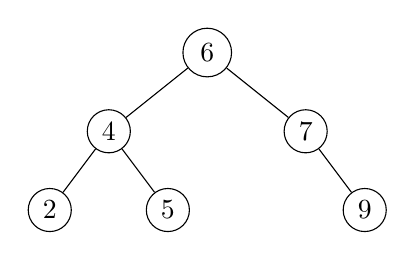
\begin{tikzpicture}
    \node [circle,draw]{6} [level distance=10mm,sibling distance=25mm]
        child { node [bstnode]{4} [level distance=10mm ,sibling distance=15mm]
        child {node [bstnode] {2}}
        child {node [bstnode] {5}}
        }
        child {node [bstnode] {7} [level distance=10mm ,sibling distance=15mm]
        child[missing]{}
        child {node [bstnode] {9}}}
        ;
\end{tikzpicture}
\end{center}

The BST property allows us to visit all the keys in a binary search tree in sorted order by a simple recursive algorithm \procedure{Inorder-Tree-Walk}.

\begin{pseudocode}{Inorder-Tree-Walk}{x}
    \IF {$x \neq \NIL$}
        \STATE \procedure{Inorder-Tree-Walk}$(x.left)$
        \STATE print $x.key$
        \STATE \procedure{Inorder-Tree-Walk}$(x.right)$
    \ENDIF
\end{pseudocode}

\vspace*{3mm}
The correctness of the algorithm follows by induction using the BST invariant. And it takes linear time to visit all the tree, proven in the following theorem.

\begin{theorem}
If $x$ is the root of an $n$-node subtree, then the call \procedure{Inorder-Tree-Walk}$(x)$ takes $\Theta(n)$ time.
\end{theorem}
\begin{proof}
Let $T(n)$ be the running time of \procedure{Inorder-Tree-Walk} when it is called on the root of an $n$-node subtree. Since \procedure{Inorder-Tree-Walk} visits all $n$ nodes of the subtree, we have that $T(n) = \Omega(n)$. It remains to prove that $T(n) = O(n)$. \\

For an empty subtree, we have $T(0) = c$, for some constant $c > 0$. For $n > 0$, suppose \procedure{Inoder-Tree-Walk} is called ona node $x$  whose left subtree has $k$ nodes and whose right subtree has $n - k - 1$ nodes. Then the runnig time is bounded by $T(n) \leq T(k) + T(n - k - 1) + d$, for some constant $d > 0$ (reflecting upper bound time to execute body of \procedure{Inorder-Tree-Walk} excluding recursive calls). By the substitution method we show that $T(n) = O(n)$ by proving that $T(n) \leq (c+ d)n + c$. \\

For $n = 0$, $T(0) = c = (c + d) \cdot 0 + c$. And for $n > 0$ we have, 
\vspace*{-1mm}
\begin{align*}
    T(n) &\leq T(k) + T(n - k - 1) + d \\
         &= ((c + d)k + c) + ((c + d)(n - k - 1) + c) + d \\
         &= (c + d)n + c,
\end{align*}
which completes the proof.
\end{proof}





\end{mysection}
